\input{../include/preamble}

\title[ID1019 Trees]{Trees}


\author{Johan Montelius}
\institute{KTH}
\date{\semester}

\begin{document}

\begin{frame}
\titlepage
\end{frame}

\begin{frame}{compound structures}

Compound data structures in Elixir:

\begin{itemize}
 \item {\bf tuples:} {\tt \{:student, ``Sune Mangs'', :cinte, 2012,  :sunem\}}
 \item {\bf lists:} {\tt [:sunem, :joed, :sueb, :anng]}
\end{itemize}
\end{frame}


\begin{frame}{lists}

We could implement lists using tuples:
 
\pause

\begin{code}
   <list> ::=  & :nil | \\
               & '\{' :cons ',' <expression> ',' <list> '\}'
\end{code}


\pause \vspace{20pt}
{\tt [:foo, :bar, :zot]}

\pause \vspace{10pt}
{\tt [:foo | [:bar | [:zot | [] ] ] ] }
 
\pause \vspace{10pt}
{\tt \{:cons, :foo, \{:cons, :bar, \{:cons, :zot, :nil\}\}\}}

\end{frame}


\begin{frame}{lists}

\pause Lists gives us a convenient syntax ... \pause once you get use to it.
\vspace{20pt}

\pause Lists are handled more efficiently by the compiler and run-time system.

\vspace{20pt}
\pause Important to understand when to use lists and when to use tuples.

\end{frame}

\begin{frame}[fragile]{n'th element}

Return the n'th element from a list of three:

\pause 
\begin{verbatim}
def nth_l(1, [r|_]) do r end
def nth_l(2, [_,r|_]) do r end
def nth_l(3, [_,_,r]) do r end
\end{verbatim}

\pause Return the n'th element from a tuple of three:
\pause

\begin{verbatim}
def nth_t(1, {r,_,_}) do r end
def nth_t(2, {_,r,_}) do r end
def nth_t(3, {_,_,r}) do r end
\end{verbatim}

\end{frame}

\begin{frame}[fragile]{nth element}

Return the n'th element from a list:

\pause 
\begin{verbatim}
def nth(1, [r|_]) do r end
def nth(n, [_|t]) do nth(n-1, t) end
\end{verbatim}

\end{frame}


\begin{frame}{nth element}

\begin{itemize}
  \item {\tt elem(tuple, n):} return the n'th element in the tuple (zero indexed)
  \item {\tt Enum.at(list, n):} return the n'th element of the list (zero indexed)
\end{itemize}

\end{frame}

\begin{frame}{n'th benchmark}
Benchmark different versions of n'th:
 \begin{figure}
  \centering
  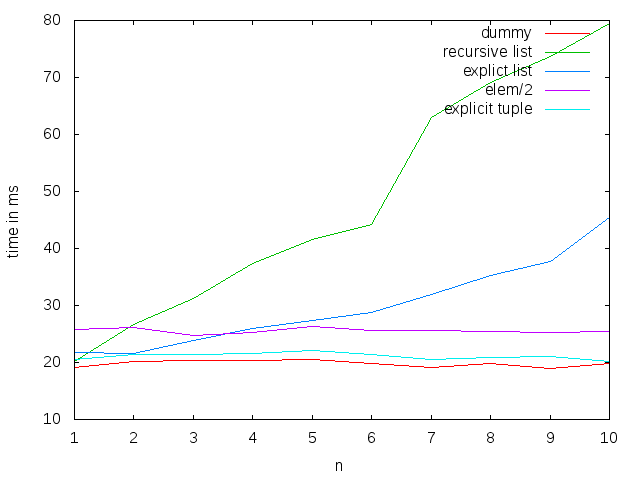
\includegraphics[height=200pt]{bench.png}
  \caption{Execution time in ms of 100.000 calls}
 \end{figure}

\end{frame}

\begin{frame}[fragile]{copying}

  Assume we represent students by a tuple {\tt \{:student, name, prgm,
    year, id\}} and we want to change the program.

\pause
\begin{verbatim}
def new_prgm({:student, name, _, year, id}, new) do \end{verbatim}\pause\begin{verbatim}
     {:student, name, new, year, id}
end
\end{verbatim}

\pause

How costly is this operations?

\vspace{10pt}
{\em Important to understand on what the cost depends on.}

\end{frame}


\begin{frame}{copying}

\end{frame}

\begin{frame}{when to use what}

Represent the following information using ether a list, tuple, number or atom.
                   
\begin{itemize}
\item a playing card: ace of club, king of hearts etc
\item a deck of playing cards
\item a car manufacturer: Volvo, Saab, Audi, \ldots
\item a year: 1984, 2001
\item a description of a car: maker, model, year
\item a phone number: +46-709757802
\item a course with an id, name, course responsible etc
\item a student with a number of courses two which she is enrolled
\end{itemize}

\end{frame}

\begin{frame}[fragile]{member of a list}

Assume we have a list of tuples {\tt \{:card, :heart, 7\}} representing playing cards. 
\pause

\vspace{10pt}
Implement a function that checks if a given card is in a deck of cards and returns {\tt :yes}, or {\tt :no}.

\begin{verbatim}
def member(_, []) do ... end
def member(card, [...|_]) do ... end
def member(card, [_|rest]) do 
    ... 
end
\end{verbatim}

\end{frame}

\begin{frame}[fragile]{trees}

\pause How do we represent a binary tree?


\vspace{10pt}
\pause How do we represent a leaf node?

\vspace{10pt}
{\tt \{:leaf, value\}}

\vspace{20pt}
\pause How do we represent a branch node?

\vspace{10pt}
{\tt \{:node, value, left, right\}}

\vspace{10pt}
\pause How do we represent an empty tree?

\vspace{10pt}
{\tt :nil}


\vspace{10pt}

\begin{verbatim}
  tree = {:node, :b, {:leaf, :a}, {:leaf, :c}}
\end{verbatim}


\end{frame}


\begin{frame}{what is happening}

{\tt t = \{:node, 38, \{:leaf, 42\}, \{:leaf, 34\}\}}

\pause \vspace{20pt}

\begin{tikzpicture}[scale=0.4]


 \leaf{10}{5}{42}
 \pause 
 \leaf{6}{3}{34}

 \pause
 \branch{0.5}{8}{38}
 \pause
 \branchleft{0.5}{8}{10}{5}
 \pause
 \branchright{0.5}{8}{6}{3}

 \node at (0,8) {{\bf t:} }; 

\end{tikzpicture}

\end{frame}

\begin{frame}{what is happening}

\begin{code}
  z = &\{:node, 40, \{:leaf, 42\} \{:leaf, 39\}\},\\
  t = &\{:node, 38, z, \{:leaf, 34\}\}
\end{code}
\pause \vspace{20pt}

\begin{tikzpicture}[scale=0.4]

 \pause 
 \:leaf{16}{6}{42}
 \pause 
 \:leaf{16}{3}{39}

 \pause 
 \branch{10}{8}{40}

 \pause
 \branchleft{10}{8}{16}{6}
 \pause
 \branchright{10}{8}{16}{3}

 \node at (9.5,8) {{\bf z:} }; 

 \pause
 \leaf{6}{3}{34}

 \pause
 \branch{0.5}{8}{38}
 \pause
 \branchleft{0.5}{8}{9}{8}
 \pause
 \branchright{0.5}{8}{6}{3}

 \node at (0,8) {{\bf t:} }; 

\end{tikzpicture}

\end{frame}


\begin{frame}[fragile]{search a tree}

Given a tree, implement a function that searches for a given number,
returning {\tt :yes} or {\tt no} depending on if the number is in the
tree or not.

\pause\vspace{20pt}

\begin{verbatim}
def member(_, :nil) do :no end
def member(n, {:leaf, ...}) do :yes end
def member(_, {:leaf, ...}) do :no end
\end{verbatim}
\pause
\begin{verbatim}
def member(n, {:node, ..., ..., ...}) do :yes end
\end{verbatim}
\pause

\begin{verbatim}
def member(n, {:node, _, left, right}) do 
          case ...  do
             :yes -> :yes
             :no -> ....
          end
end
\end{verbatim}

\pause\vspace{20pt}
What is the asymptotic time complexity of this function?
\end{frame}


\begin{frame}[fragile]{ordered tree}

How is the situation changed if the tree is ordered?

\pause\vspace{10pt}

\begin{verbatim}
def member(_, :nil) do :no end
def member(n, {:leaf, ...}) do :yes end
def member(_, {:leaf, ...}) do :no end
def member(n, {:node, ..., ..., ...}) do :yes end
\end{verbatim}
\pause
\begin{verbatim}
def member(n, {:node, v, left, right}) do 
          if  n < v do
             ...
          else 
              ...
          end
end
\end{verbatim}

\pause{\em What is the asymptotic time complexity of this function?}

\end{frame}

\begin{frame}{key-value look-up}
Assume that we have an ordered tree of key-value pairs:

\begin{code}
  t = \{:node,&:k, 38,\\
             &\{:node, b, 34,&:nil, :nil\},\\
             &\{:node, o, 40,&\{:node, :l, 42, :nil, :nil\}, \\
                           &&\{:node, :q, 39, :nil, :nil\}\}\}\\

\end{code}

\vspace{20pt}No special leaf nodes, empty branch is represented by {\tt :nil}.

\end{frame}

\begin{frame}[fragile]{lookup in order tree}

\pause\vspace{10pt}
How would we implement a function that searched for a given key and
returned {\tt \{:value, value\}} if found and {\tt :no} otherwise?
\vspace{20pt}\pause

\begin{verbatim}
def lookup(key, :nil) do ... end
\end{verbatim}
\pause
\begin{verbatim}
def lookup(key, {:node, key, ..., ..., ...}) do ... end
\end{verbatim}
\pause
\begin{verbatim}
def lookup(key, {:node, k, _, left, right}) do 
          if key < k do
               ... 
          else 
               ...
          end
end
\end{verbatim}


\end{frame}



\begin{frame}[fragile]{modify an element}

\begin{verbatim}
def modify(_, _, :nil) do :nil end
\end{verbatim}
\pause
\begin{verbatim}
def modify(key, val, {:node, key, _, left, right}) do 
    {:node, key, val, left, right}
end
\end{verbatim}
\pause
\begin{verbatim}
def modify(key, val, {:node, k, v, left, right}) do 
    if key < k do
        {:node, k, v, ..., right};
    else
        {:node, k, v, left, ...}
    end
end
\end{verbatim}

\end{frame}


\begin{frame}[fragile]{insert}

Same assumptions, how do we implement {\tt insert(key, value, tree)} (assuming it does not exists)?

\pause\vspace{20pt}

\begin{verbatim}
def insert(key, value, :nil) do ...    end
\end{verbatim}
\pause
\begin{verbatim}
def insert(key, value, {:node, k, v, left, right}) do 
          if key < k do
              ... 
          true -> 
              ...
          end
\end{verbatim}

\end{frame}


\begin{frame}[fragile]{delete}

Same assumptions, how do we implement {\tt delete(Item, Tree)} (assuming it does exists)?

\pause\vspace{20pt}

\begin{verbatim}
def delete(key, {:node, key, _, :nil, :nil}) do ... end
\end{verbatim}
\pause
\begin{verbatim}
def delete(key, {:node, key, _, :nil, right}) do ... end
\end{verbatim}
\pause
\begin{verbatim}
def delete(key, {:node, key, _, left, :nil}) do ... end
\end{verbatim}
\pause
\begin{verbatim}
def delete(key, {:node, key, _, left, right}) do end
            :
\end{verbatim}
\pause
\begin{verbatim}
def delete(key, value, {:node, k, v, left, right}) do 
          if key < k do
               ...
          else
               ...
          end
end
\end{verbatim}
\end{frame}

\begin{frame}[fragile]{deleting a element}

\pause Algorithm first - then implement.

\pause
\begin{verbatim}
def delete(key, {:node, key, _, left, right}) do 
         {k, v} = ....
         deleted = ...
         {:node, ..., ..., ..., ...}
end
\end{verbatim}

\end{frame}



\begin{frame}{Summary}

\vspace{40pt}\hspace{80pt}Trees

\end{frame}


\end{document}


